% NOTE : COMMENT ON TRACE LE DEPLACREMENT -> MOYENNE AU NOEUDS A PRECISER DANS LA LEGENDE DE LA FIGURE
% NOTE : LE CODE, CE QU'ON UTILISE, MFRONT MGIS -> IMPLEMENTATION PORTEE DANS CAST3M -> IMPLEMENTATION PLUGGABLE DANS AUTRE CHOSE -> 
% NOTE : ON PARLE PAS DES TEMPS DE CALCULS DANS LA SUITE parce que c du python, on montr que les 2 schémas d'intégration convergecne de manière qudartique, localement et globalement
% POUR ETRE COHERENT EN CONDENSATION, IL FAUT ACCLERER LES FACES +  LES CELLULES. POUR NOUS C QUE LES FACES


% ---------------------------------------------------------
% ---- SECTION
% ---------------------------------------------------------
\section{Numerical examples in the axisymmetric modelling hypothesis}
\label{sec_numerical_examples}

In this section, we evaluate the proposed axi-symmetric HHO method on
classical test cases taken from the literature to emphasize robustness
to volumetric locking. We consider both the small and large strains
framework, for elasto-plastic behaviors. In this section, we denote by
HHO($k,l$) the HHO element of order $k$ on faces, and order $l$ in the
cell.

The tests presented in this section have been performed using an
\texttt{python} implementation freely available on github: \url{...}.
The results of this implementations were toroughly compared to the
results obtained with the reference implementation provided the
\texttt{Disk++} solver.

% ---------------------------------------------------------
% PARAGRAPH
% ---------------------------------------------------------
\paragraph{Stabilization parameter}

To ensure coercivity of the HHO method, the stabilization parameter
$\beta$ needs be chosen according to the material under study. In the
literature~\cite{di_pietro_discontinuous-skeletal_2015}, a value of
order $2 \mu$ is advocated, where $\mu$ denotes the shear modulus of the
material. We use this values for all test cases in the present section.

% ---------------------------------------------------------
% -- SUBSECTION
% ---------------------------------------------------------
\subsection{The free dilatation test}
\label{sec_satoh_test}

The first test case of the following benchmark aims at displaying the
robustness of the HHO method for coupled mechanical-thermal problems.

% ---------------------------------------------------------
% PARAGRAPH
% ---------------------------------------------------------
\paragraph{Specimen and loading}

For this test case, the unit box is fixed on both the right and
bottom boundaries in their respective normal directions, and a quadratic
thermal load depending on the $r$-coordinate is imposed in the solid
(see Figure \ref{fig_satoh_setting}). The mesh is composed of 400
quadrangles. The thermal loading is given by:
%
%
%
\begin{equation}
    T(r,z) = 4 (T_{max} - T_{min})r(1 - r) + T_{min}
\end{equation}
%
%
%
with temperature values $T_{max} = 2000$ K and $T_{min} = 293.15$ K.

\begin{figure}[H]
    \centering
    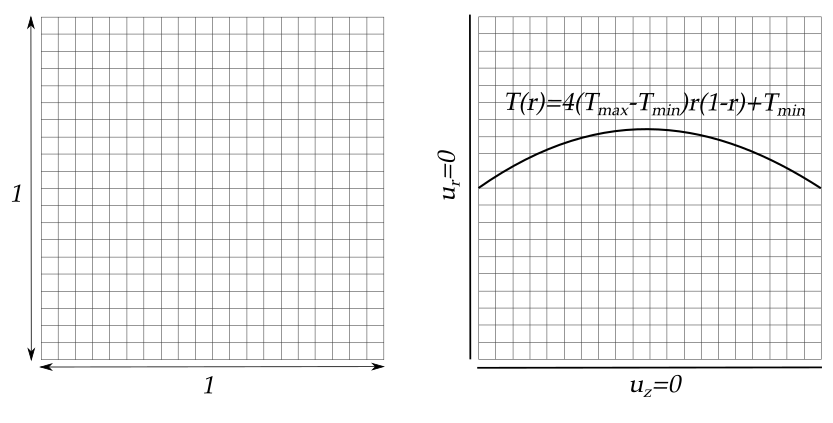
\includegraphics[width=10.cm]{img_calcs/satoh_setting.png}
    \caption{Geometry, displacement boundary conditions and temperature loading for the free dilatation test case}
    \label{fig_satoh_setting}
\end{figure}

% ---------------------------------------------------------
% PARAGRAPH
% ---------------------------------------------------------
\paragraph{Material behaviour}

A linear thermo-elastic energy potential is considered with a Young's
modulus $E$ equal to $150$ GPa. The material is quasi-incompressible
with a Poisson's ratio $\nu$ equal to $0.499$. The dilatation parameter
is taken as $\alpha = 1e^{-6}$ K$^{-1}$.

% ---------------------------------------------------------
% PARAGRAPH
% ---------------------------------------------------------
\paragraph{Volumetric locking and polynomial approximation for the strain and temperature fields}

Lagrange finite elements of order $1 \leq k \leq 2$ evaluate a
mechanical strain of order $0 \leq k-1 \leq 1$, whereas the thermal
strain is of order $2$. Using the total strain for the computation of
the stress results in strong volumetric locking. Hence, for Lagrange
element to accurately model the problem, one needs to choose a
temperature fields that is one order lower than that describing the
displacement field. This feature is of major importance for mixed
elements, where quadratic elements needs be employed to match the the
linear pressure unknown polynomial order.

\begin{figure}[H]
    \centering
    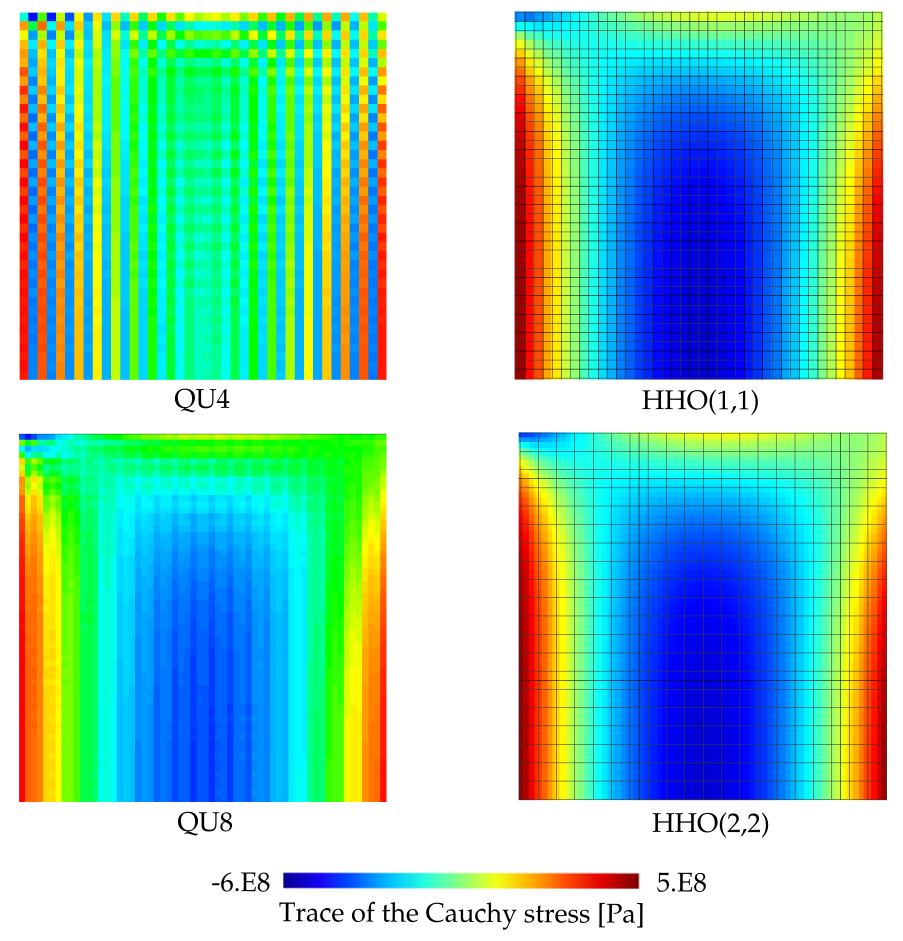
\includegraphics[width=10.cm]{img_calcs/satoh_calc.png}
    \caption{Map fo the Trace of the Cauchy stress at quadrature points for the Free dilatation test case at the last time step}
    \label{fig_satoh_calc}
\end{figure}

% ---------------------------------------------------------
% PARAGRAPH
% ---------------------------------------------------------
\paragraph{Comparison of FE and HHO methods}

In Figure \ref{fig_satoh_calc}, one can observe that the pressure map is completely smooth for the HHO computations, even for a quadratic temperature field acting on a linear gradient using HHO(1,1). As expected, the results display mild signs of volumetric locking for the quadratic finite element
approximation, and strong oscillations are noted for the linear finite element solution.

% ---------------------------------------------------------
% -- SUBSECTION
% ---------------------------------------------------------
\subsection{Perfect plastic swelling sphere}
\label{sec_swelling_sphere}

% ---------------------------------------------------------
% PARAGRAPH
% ---------------------------------------------------------
\paragraph{Specimen and loading}

This benchmark consists in a quasi-incompressible sphere under uniform internal loading.
This test case has an analytical solution and the state of the specimen is known when the plastic region has reached the external border of the sphere.
The sphere has an inner radius $r_{int} = 0.8$ mm and an outer
radius $r_{ext} = 1$ mm. An internal radial displacement $u$ is imposed. The mesh is composed of XXX quadrangles (see Figure \ref{fig_sphereall}).
The simulation is performed until the limit load corresponding to an internal displacement of $0.2$ mm is reached.

% ---------------------------------------------------------
% PARAGRAPH
% ---------------------------------------------------------
\paragraph{Material behaviour}

An isotropic hardening energy potential $\mecPotential{}_{\bodyLag{}}^p$ is chosen for the description of the plastic evolution of the material such that

\begin{equation}
    \mecPotential{}_{\bodyLag{}}^p(p)
    =
    \sigma_0 p + \frac{1}{2} H p^2 + (\sigma_{\infty} - \sigma_0)(p - \frac{1 - e^{-\delta p}}{\delta})
\end{equation}
%
%
%
where the parameter $p$ denotes the equivalent plastic strain and a Von Mises yields function $f$ describes the flow rule
%
%
%
\begin{equation}
    f = \sqrt{\frac{3}{2}} \rVert \text{dev} (\tensorii{\sigma}) \lVert - p
\end{equation}
%
%
%
Moreover, the small strain hypothesis is assumed for this test case.
Perfect plasticity is considered for this test case , where the saturation parameter $\delta = 0$, the yield stresses $\sigma_0 = \sigma_{\infty} = 6$ MPa, the hardening parameter $H = 0$ and the elastic potential parameters are the Young modulus $E = 28.85$ MPa and the Poisson ratio $\nu = 0.499$, such that the material is quasi-incompressible.

\begin{figure}[H]
    \centering
    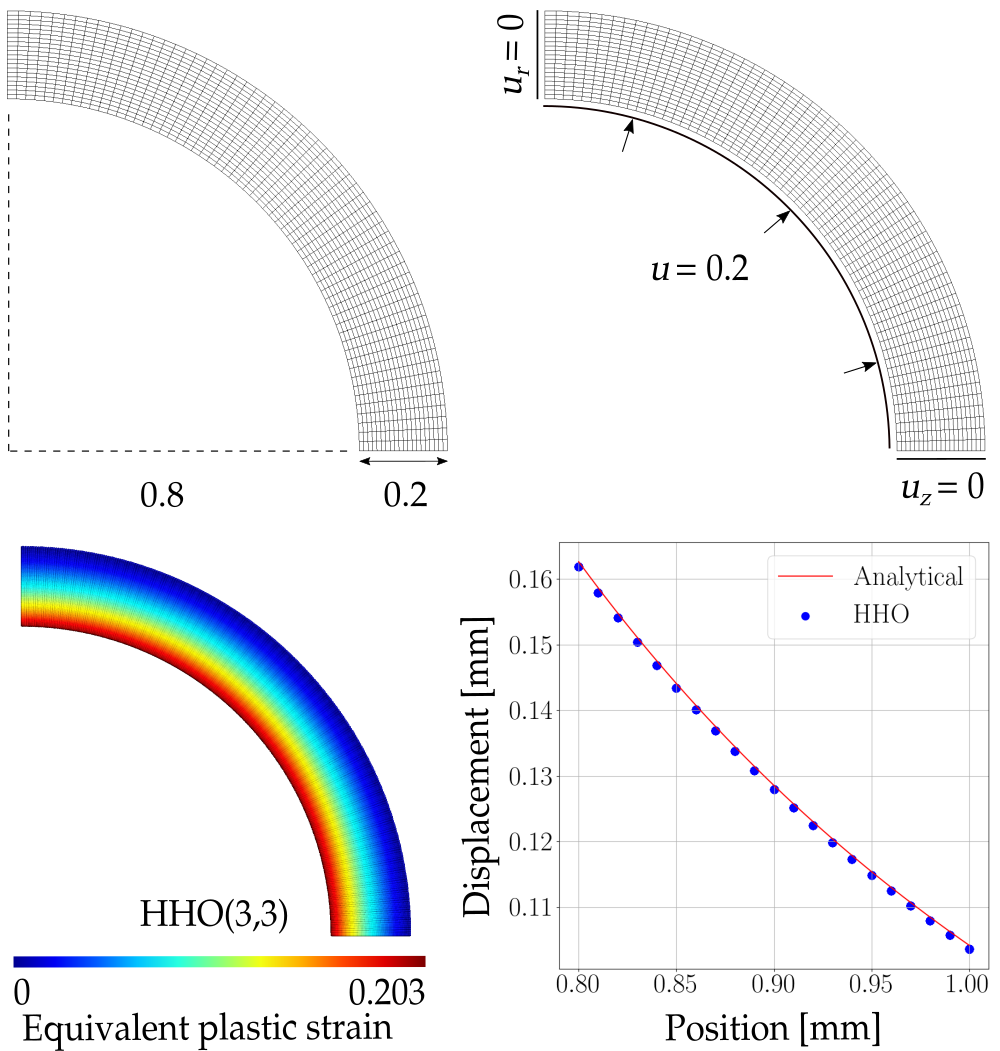
\includegraphics[width=12.cm]{img_calcs/sphere_mesh.png}
    \caption{the swelling sphere test case. Geometry, loadings, final displacement along the radius of the sphere, and final equivalent plastic strain map at quadrature points}
    \label{fig_sphereall}
\end{figure}

% ---------------------------------------------------------
% PARAGRAPH
% ---------------------------------------------------------
\paragraph{Displacement along the radius}

Since an analytical solution is known for this test case, we compare it to the proposed HHO method. The displacement of the section of the sphere at cell nodes
is plotted in Figure \ref{fig_sphereall}, along with the analytical one, and we observe that the obtained results are in agreement with the analytical response.
Figure \ref{fig_sphereall} mentions the label HHO without specifying approximation orders for all computations deliver the same result.

% ---------------------------------------------------------
% PARAGRAPH
% ---------------------------------------------------------
\paragraph{Trace of the Cauchy stress}

As for the displacement, the analytical solution for the trace of the Cauchy stress tensor is compared to the one computed using the proposed HHO method for three approximation orders.
A sign of volumetric locking is the presence of strong oscillations in the trace of the Cauchy stress (or, equivalently, the hydrostatic pressure) within elements.
We observe that numerical results at quadrature points fit the analytical curve, and display no sign of volumetric locking. The computed solution is however less smooth
at the borders of the specimen for higher orders, a phenomenon that was pointed out in \cite{abbas_hybrid_2019-1} for the three dimensional case, and attributed to the fact that planar faces are considered.

\begin{figure}[H]
    \centering
    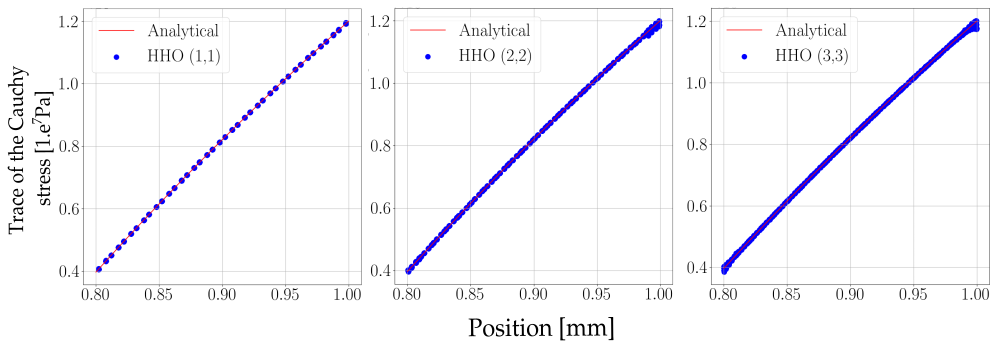
\includegraphics[width=15.cm]{img_calcs/sphere_pressures.png}
    \caption{trace of the Cauchy stress tensor along the radius of the sphere at quadrature points}
    \label{fig_sphere_pressure}
\end{figure}

% ---------------------------------------------------------
% -- SUBSECTION
% ---------------------------------------------------------
\subsection{Necking of a notched bar}

% ---------------------------------------------------------
% PARAGRAPH
% ---------------------------------------------------------
\paragraph{Specimen and loading}

We consider a notched bar that is subjected to uniaxial
extension.
The bar has a length of $30$ mm, a top section of radius $5$ mm and a bottom section of radius $3$ mm.
A vertical
displacement $u_z = 0.8$ mm is imposed at the top, as shown in Figure \ref{fig_ssnaallmesh}.
For symmetry reasons, only one-quarter of the
bar is discretized, and the mesh is composed of XXX quadrangles.

% ---------------------------------------------------------
% PARAGRAPH
% ---------------------------------------------------------
\paragraph{Behaviour law}

The same behavior law as that in \ref{sec_swelling_sphere} is considered for the present test case. 
However, the finite strain hypothesis is chosen, based on a logarithmic decomposition of the stress \cite{miehe_anisotropic_2002}.

% ---------------------------------------------------------
% PARAGRAPH
% ---------------------------------------------------------
\paragraph{Material parameters}

Materials parameters are taken as
$\sigma_0 = 450$ MPa, $\sigma_{\infty} = 715$ MPa with a saturation parameter $\delta = 16.93$. The Young modulus is $E = 206.9$ GPa, and the Poisson ratio is $\nu = 0.29$.

% ---------------------------------------------------------
% PARAGRAPH
% ---------------------------------------------------------
\paragraph{Load deflection curve}

The load-displacement curve is plotted
in Figure \ref{fig_ssnaallmesh}, and gives similar results to that obtained with quadratic reduced integration elements.

% ---------------------------------------------------------
% PARAGRAPH
% ---------------------------------------------------------
\paragraph{Equivalent plastic strain}

Moreover, the equivalent
plastic strain $p$ at quadrature points and at the final load is plotted Figure \ref{fig_ssnaallplastic}.
It has been observed that the equivalent plastic strain might suffer some oscillations at a certain limit load with UPG methods.
One notices through the present example, that the proposed HHO method displays no oscillations of the equivalent plastic strain.

\begin{figure}[H]
    \centering
    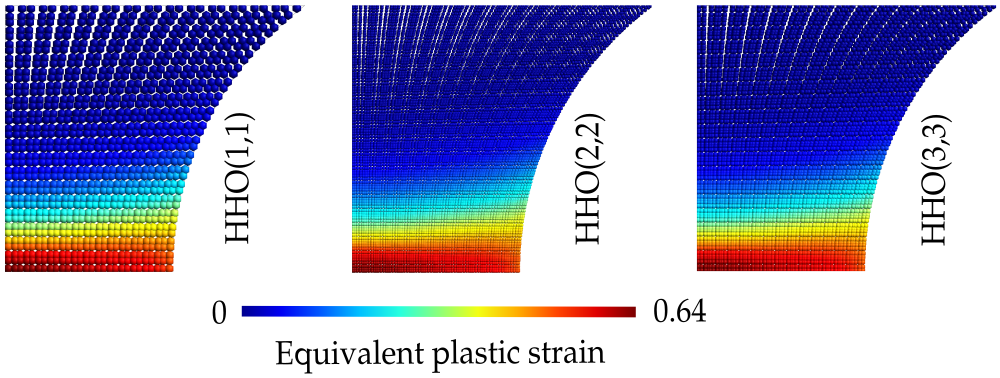
\includegraphics[width=12.cm]{img_calcs/ssna_plastic.png}
    \caption{
        final equivalent plastic strain map at quadrature points in the notch region
    }
    \label{fig_ssnaallplastic}
\end{figure}

% ---------------------------------------------------------
% PARAGRAPH
% ---------------------------------------------------------
\paragraph{Hydrostatic pressure}

The hyrostatic pressure map at quadrature points and at the final load is shown Figure \ref{fig_ssnaallmesh} for three HHO element orders (respectively $1, 2$ and $3$).
As for the swelling sphere test case, one notices that the hydrostatic pressure map is
fairly smooth over the whole structure at all approximation orders, even at the bottom left corner where plasticity is confined.

\begin{figure}[H]
    \centering
    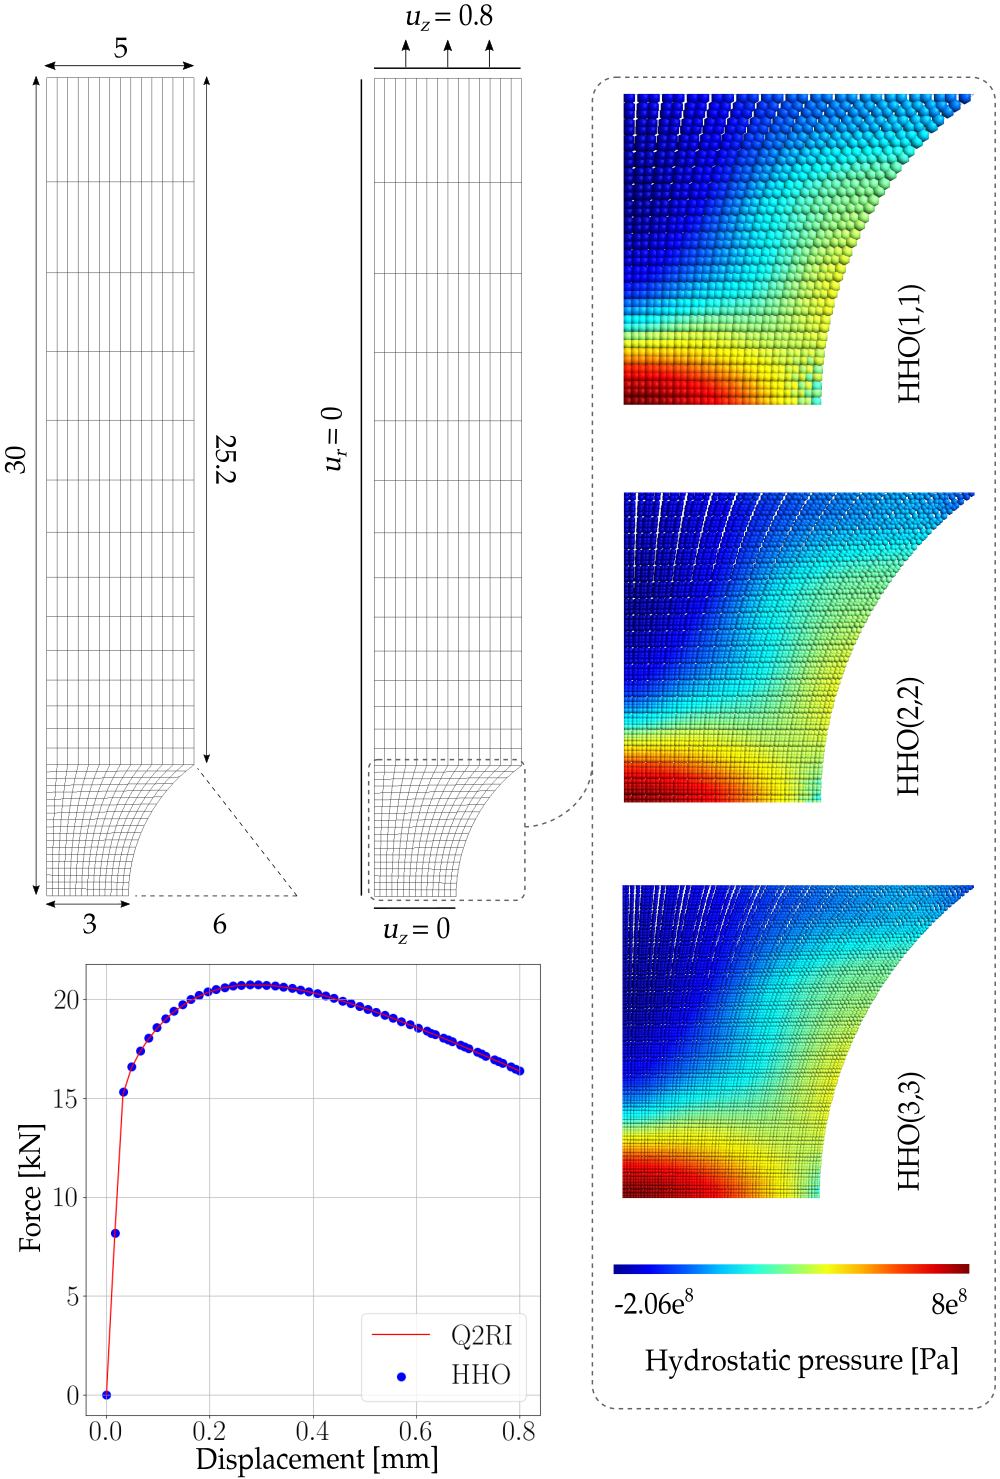
\includegraphics[width=12.cm]{img_calcs/ssna_mesh.png}
    \caption{
        the notched specimen test case. Geometry, loadings, load deflection curve, and final hydrostatic pressure map at quadrature points in the notch region
    }
    \label{fig_ssnaallmesh}
\end{figure}

% ---------------------------------------------------------
% ---- SECTION
% ---------------------------------------------------------
\section{Numerical examples in plane strain and tridimensional modelling hypotheses}
\label{sec_num_example_part_2}

The section showcases numerical examples demonstrating the robustness
of the cell resolution algorithm. The test cases under study, namely the
classical Cook membrane, and the indentation test cases, show that no
volumetric locking is encountered using the cell resolution algorithm.

% ---------------------------------------------------------
% -- SUBSECTION
% ---------------------------------------------------------
\subsection{Cook's membrane test case}

% ---------------------------------------------------------
% PARAGRAPH
% ---------------------------------------------------------
\paragraph{Specimen and loading}

Let consider the Cook membrane specimen that is subjected to uniaxial
traction. The membrane has a width of $48$ mm and a height of $60$ mm,
and a vertical traction $t_y = 1000$ N/m is imposed at the top. The HHO
computation is run on a polygonal mesh (see Figure \ref{fig_cook}) and
is compared with standard QU4 and QU8 formulations (\textit{i.e.} linear
and quadratic approximations)

% ---------------------------------------------------------
% PARAGRAPH
% ---------------------------------------------------------
\paragraph{Constitutive equation}

The same behavior law as that in \ref{sec_swelling_sphere} is
considered for the present test case. However, the finite strain
hypothesis is chosen, based on a logarithmic decomposition of the stress
\cite{miehe_anisotropic_2002}.

% ---------------------------------------------------------
% PARAGRAPH
% ---------------------------------------------------------
\paragraph{Material parameters}

Materials parameters are taken as
$\sigma_0 = 450$ MPa, $\sigma_{\infty} = 715$ MPa with a saturation parameter $\delta = 16.93$. The Young modulus is $E = 206.9$ GPa, and the Poisson ratio is $\nu = 0.29$.

\begin{figure}[H]
    \centering
    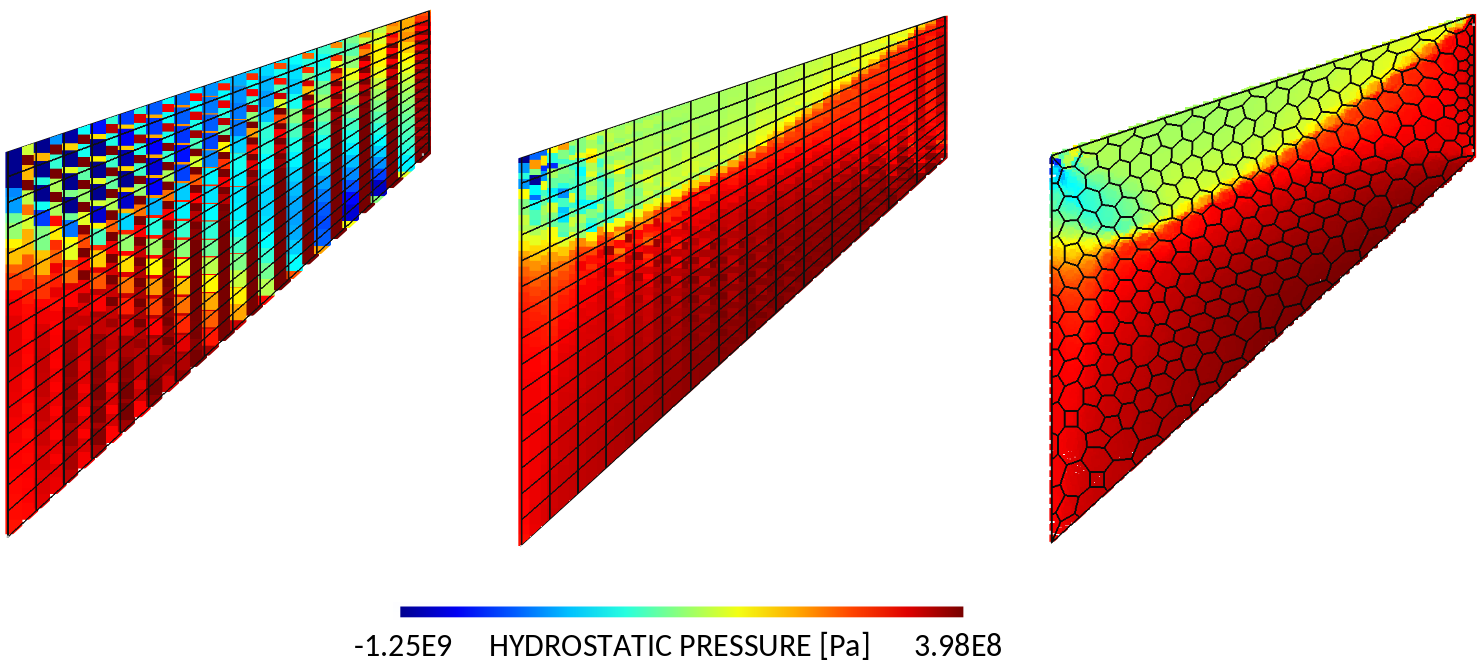
\includegraphics[width=12.cm]{img_calcs/cook_comp.png}
    \caption{Hydrostatic pressure map one the reference configuration at the limit load}
    \label{fig_cook}
\end{figure}

% ---------------------------------------------------------
% PARAGRAPH
% ---------------------------------------------------------
\paragraph{Numerical results}

As expected, the linear and quadratic finite element methods display respectively strong and mild oscillations of the pressure, whereas the HHO one shows no sign of locking.

% ---------------------------------------------------------
% -- SUBSECTION
% ---------------------------------------------------------
\subsection{Indentation test case}

% ---------------------------------------------------------
% PARAGRAPH
% ---------------------------------------------------------
\paragraph{Specimen and loading}

The last test case consists in the indentation of a cube of size $10$ mm. A pressure of $300$ MPa is imposed on the top surface see Figure \ref{fig_cube}).

% ---------------------------------------------------------
% PARAGRAPH
% ---------------------------------------------------------
\paragraph{Material}

The same perfect plastic material as that in \ref{sec_swelling_sphere} is considered for the present test case.

\begin{figure}[H]
    \centering
    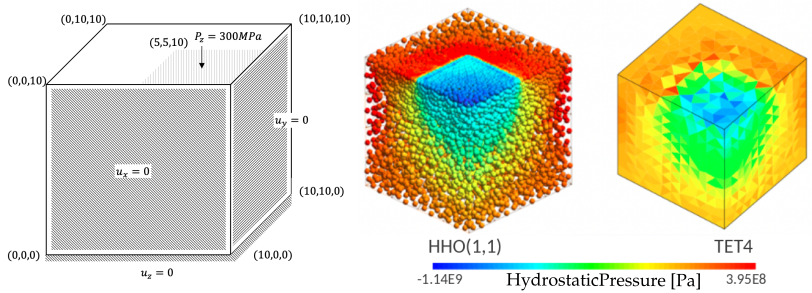
\includegraphics[width=12.cm]{img_calcs/cube.png}
    \caption{Hydrostatic pressure map one the reference configuration at the limit load}
    \label{fig_cube}
\end{figure}

% ---------------------------------------------------------
% PARAGRAPH
% ---------------------------------------------------------
\paragraph{Numerical results}

The pressure map at the end of the computation is displayed in Figure \ref{fig_cube}, and no sign of volumetric locking are present on the HHO computation, as opposed to the linear finite element one.